        %auto-ignore
\section{Block Depth 2 and Above}

\label{sec:bd2}

\emph{Remark on notation:} Here and in the next section, all big-O notation is in $L$ only; the scaling in width is assumed to be in $\mu$P.

In most of this work, we have considered depth-1 MLP for $g^l$ in \cref{eqn:resmlp_defn}, it's straightforward to derive and classify the infinite-width-then-infinite-depth limits for larger depths in each block.
In particular, the following $1/\sqrt{L}$ scaling still makes sense in this more general setting with block depth $k$ and leads to a well defined limit:

    \begin{align}
        x^{l}&=x^{l-1} +\frac a {\sqrt L} \cdot g^l(x^{l-1}; W^{l1}, \ldots, W^{lk}),\quad\text{$\Theta(1)$ initialization scale,}\quad\text{$\Theta(1/\sqrt L)$ learning rate}
    \end{align}
This is what we call Depth-$\mu$P in the block depth 1 case, but we shall not use this name in the general block depth case because \emph{this parametrization is no longer optimal}.\footnote{What we exactly mean by \emph{optimal} will be explained below.}

\subsection{Block Depth $\ge 2$ is Defective}

A very clear symptom of this is that the \emph{performance of block-depth-2 resnets is worse than that of block-depth-1 networks}, when matching parameter count, although they can (but not always) catch up after training for a long time (\cref{fig:relu-ln0-compare-bd,fig:abs-ln1-bd1-vd-bd2}).
\begin{figure}
    \centering
    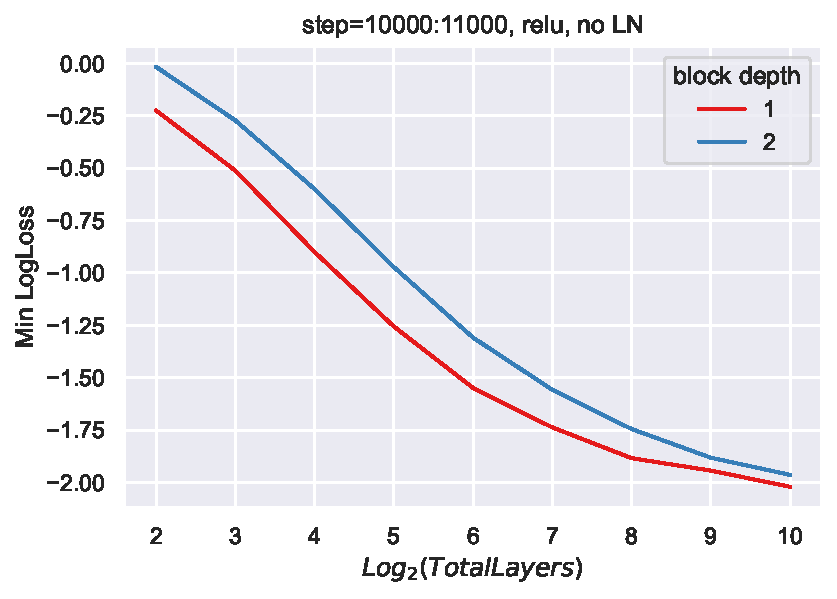
\includegraphics[width=0.4\linewidth]{fig/relu-ln0-compare-bd-10000.pdf}
    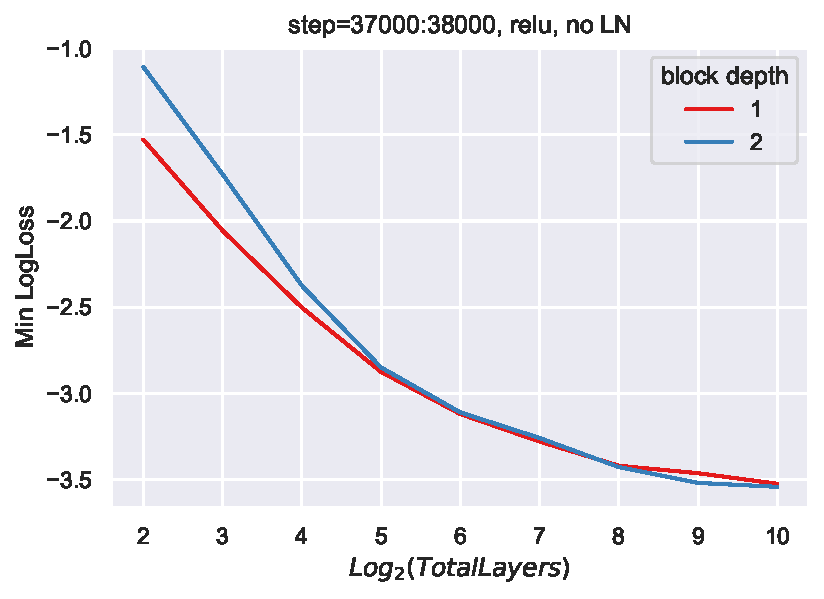
\includegraphics[width=0.4\linewidth]{fig/relu-ln0-compare-bd-37000.pdf}
    \caption{\textbf{Block Depth 2 < Block Depth 1, Relu}. In relu resnet with no LN, block depth 2 does worse than block depth 1 when matching total number of layers (and thus parameter count). However, training longer (38000 steps, Right) helps it catch up (compared to 11000 steps, Left). The y-axis is minimal log loss over all block multiplier and learning rate}
    \label{fig:relu-ln0-compare-bd}
\end{figure}
\begin{figure}
    \centering
    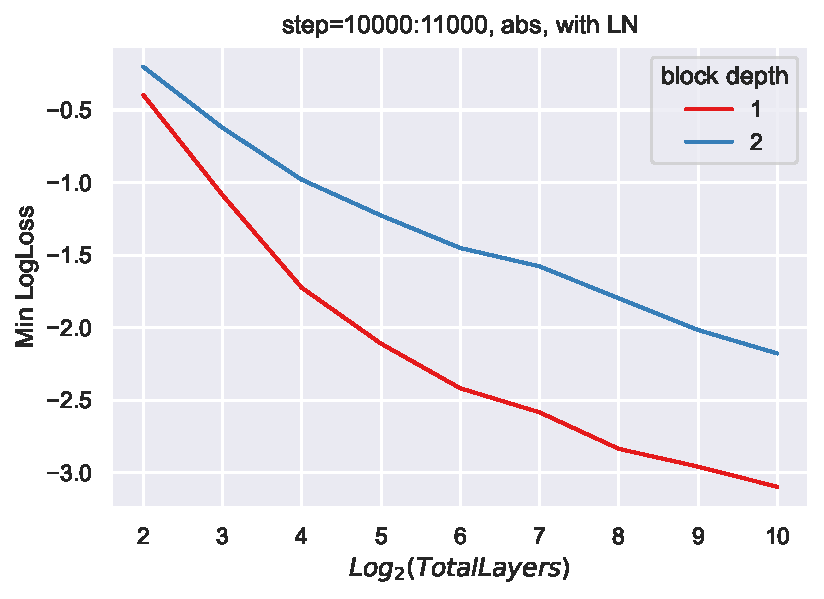
\includegraphics[width=0.4\linewidth]{fig/abs-ln1-compare-bd-10000.pdf}
    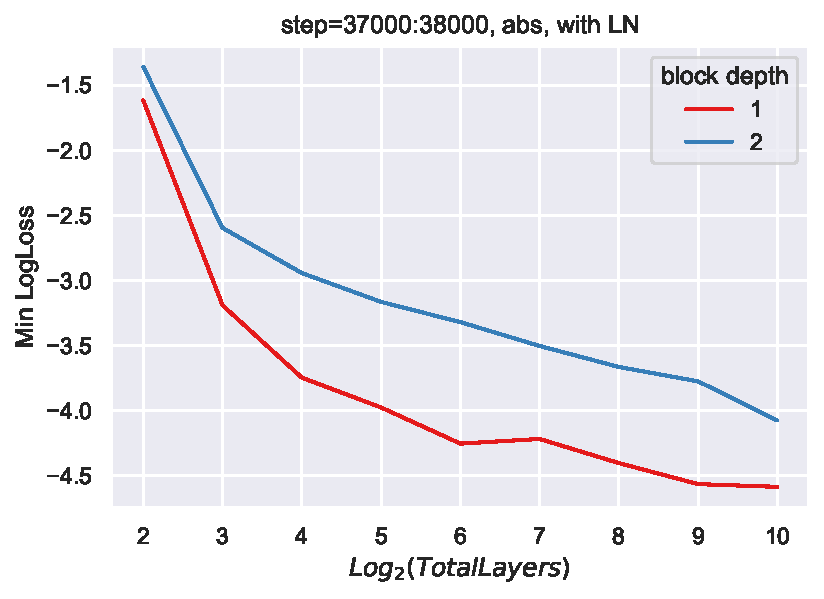
\includegraphics[width=0.4\linewidth]{fig/abs-ln1-compare-bd-37000.pdf}
  \caption{\textbf{Block Depth 2 < Block Depth 1, Abs}. In abs resnet with LN, block depth 2 does significantly worse than block depth 1 when matching total number of layers (and thus parameter count). Training longer (38000 steps, Right) does not close the performance gap (compared to 11000 steps, Left). The y-axis  is minimal log loss over all block multiplier and learning rate}
    \label{fig:abs-ln1-bd1-vd-bd2}
\end{figure}
Simultaneously, we are seeing nontrivial or even significant hyperparameter shifts as the total number of blocks increases (\cref{fig:bd2-hp-shift}).
\begin{figure}
    \centering
    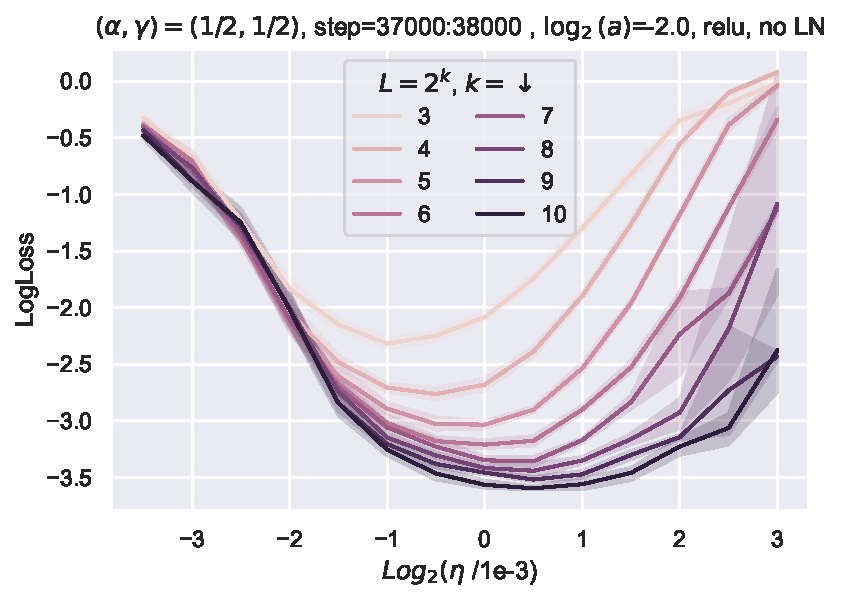
\includegraphics[width=0.4\linewidth]{fig/relu_ln0_bd2_mup_37000.pdf}
    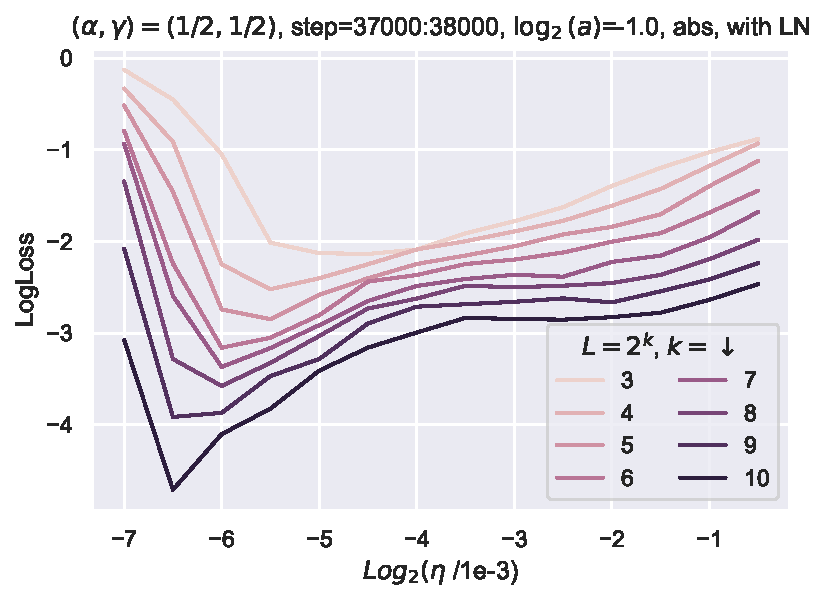
\includegraphics[width=0.4\linewidth]{fig/abs_ln1_bd2_mup_37000.pdf}
    \caption{\textbf{Block Depth 2 Hyperparameter Shift} in relu resnet with no LN (Left) and abs resnet with LN (Right).}
    \label{fig:bd2-hp-shift}
\end{figure}

\subsection{Defect of $1/\sqrt L$  Scaling in Block Depth 2}

The reason that the $1/\sqrt L$ scaling is no longer fine in the block depth $\ge 2$ case is the \emph{linearization of the multiplicative interaction} between the layers in the block.
Indeed, just like the block depth 1 case, the $1/\sqrt L$ scaling forces the weight updates $\Delta W$ of each weight matrix to be $\Theta(\sqrt{L})$ smaller than the initialization $W_0$.
Thus, within the block, the training dynamics when depth $L$ is large is in the kernel regime, where the contribution to the block output $g(x; W^\bullet)$ is only a \emph{summation}, instead of \emph{product}, of individual contributions from each layer's weights updates.

When aggregated over all $L$ blocks, the result is that there is only multiplicative interaction of $\Delta W$ across blocks but not within layers.
In other words, the network output is dominated, for example in the linear case, by the contributions of the form
$M^L \cdots M^1$
where each $M^l$ can be one of $I, W_0^{l2} W_0^{l1}, W_0^{l2} \Delta W^{l1},$ or $\Delta W^{l2} W_0^{l1}$, but NOT $\Delta W^{l2} \Delta W^{l1}$.
All other contributions (which all involve within-block interactions like $\Delta W^{l2} \Delta W^{l1}$) are subleading. 
In the general nonlinear case, replacing the block 
\begin{equation*}
    \phi(W^{l2}\phi(W^{l1} x^{l-1}))    
\end{equation*}
with the linearized version 
\begin{equation*}
    \phi(h^l_\wedge) + \phi'(h^l_\wedge) \odot [\Delta W^{l2}\phi(h^l_\vee)] + \phi'(h^l_\wedge) \odot [W_0^{l2} (\phi'(h^l_\vee) \odot [\Delta W^{l1} x^{l-1}])]    
\end{equation*}
will achieve the same performance as depth $L \to \infty$,
where $h^l_\wedge = W_0^{l2}\phi(h^l_\vee)$ and $h^l_\vee = W_0^{l1} x^{l-1}$.

When block depth $k=1$ (our main subject of study in this work), \emph{all} interactions are included but this is no longer true when $k>1$.

In \cref{fig:bd2_shifting_slope}, the heatmap of loss as a function of block multiplier and learning rate demonstrates this vividly for block depth 2.

\paragraph{Small depth}
The optimal sublevel set of (learning rate, block multiplier) has slope $\approx -2$ when the number of blocks is $2^1$. In other words, around the optimum, double the learning rate while dividing the block multiplier by 4 has similar performance. This is because $\Delta W^{l1}$ and $\Delta W^{l2}$ interact \emph{multiplicatively}, so that doubling their sizes leads to quadrupling their contribution to the block output. The simultaneous decrease of block multiplier by 4 then roughly keep their contribution invariant in size.

\paragraph{Large depth}
On the other hand, the optimal sublevel set has slope $\approx -1$ when the depth is $2^{10}$: Doubling the learning rate while halving the block multiplier has similar performance. This reflects the fact that  $\Delta W^{l1}$ and $\Delta W^{l2}$ now interact \emph{additively}. 

Intermediate depths interpolate this phenomenon, as seen in the plot for depth $2^5$.
\begin{figure}
    \centering
    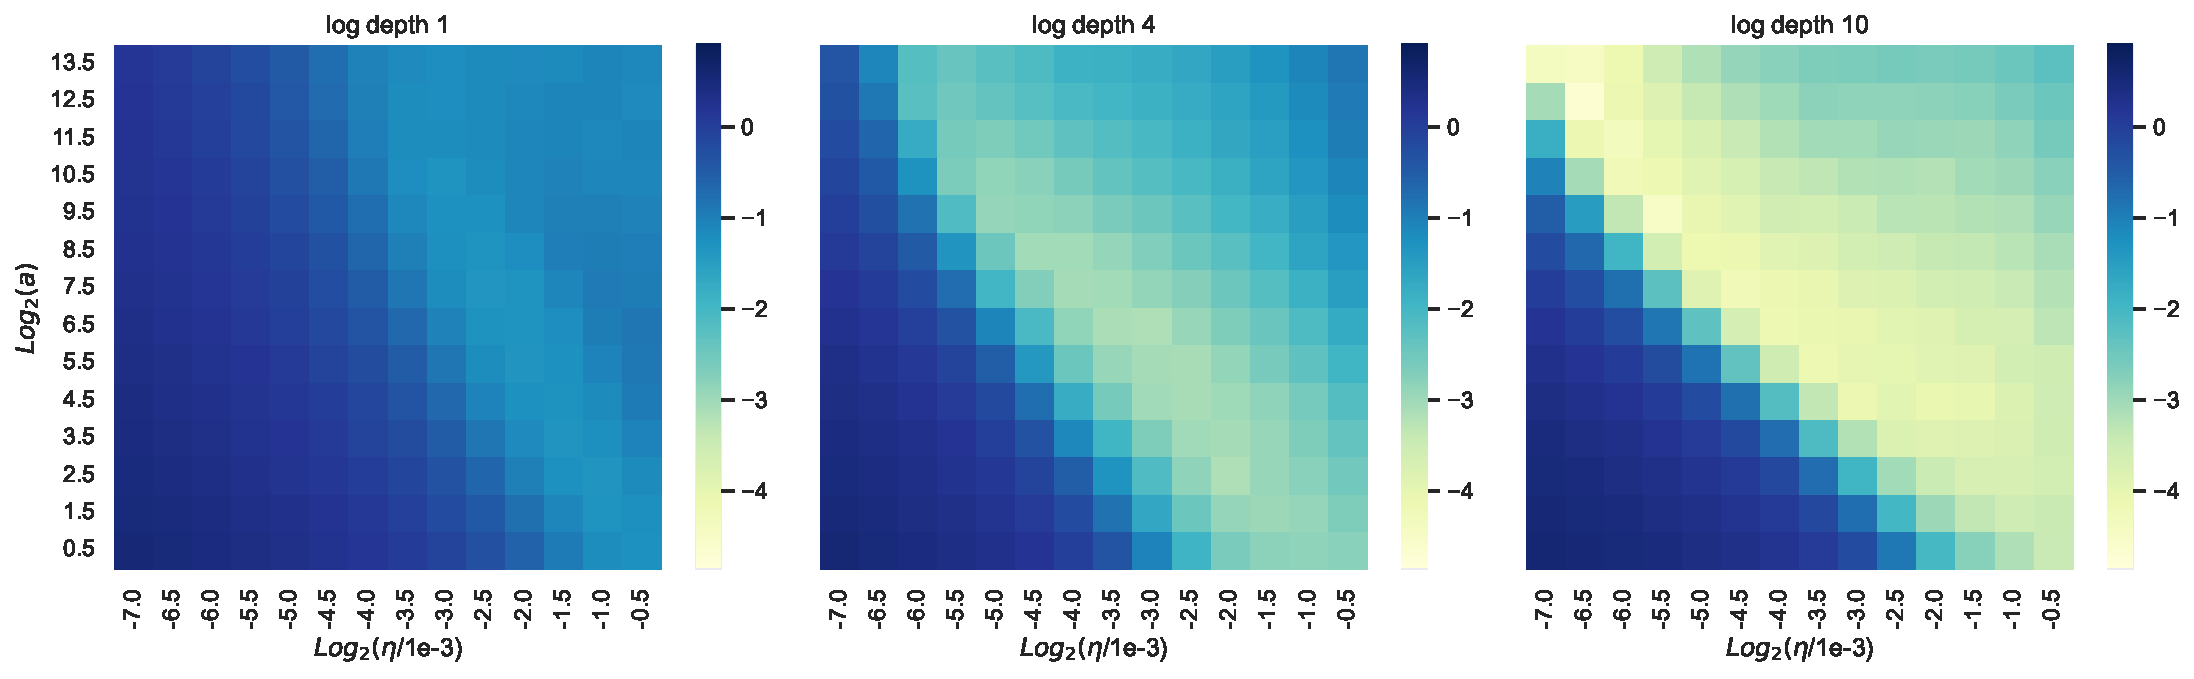
\includegraphics[width=0.9\linewidth]{fig/bd2_shifting_slope.pdf}
    \caption{The "slope" of the optimal sublevel set in the (learning rate, block multiplier) space changes from $-2$ to $-1$ as depth goes from $2^1$ to $2^{10}$. Here we use absolute value nonlinearity with layer normalization, block depth 2, and networks are trained for 50 epochs with Adam on CIFAR-10.} 
    \label{fig:bd2_shifting_slope}
\end{figure}

In the same heatmaps, one can see the optimal (learning rate, block multiplier) (in the $1/\sqrt L$ parametrization) shifts from the middle of the grid to the upper left as depth goes from $2^5$ to $2^{10}$, demonstrating the lack of hyperparameter transfer.

This change in slope is seen in relu networks as well, with or without layernorm.

Finally, we note that the $1/\sqrt{L}$ scaling still yields a $L \to \infty$ limit where the network still learns features as a whole, even though within each block this is no longer true.
Thus, this is another reminder that mere "feature learning" does not imply "hyperparameter transfer"!

\subsection{Classification of Parametrizations}

These heatmaps already demonstrate that no parametrization of (global learning rate\footnote{meaning, the learning tied across all layers in a block}, block multiplier) can transfer hyperparameters robustly, because any such parametrization can only \emph{shift} the heatmaps but not \emph{stretch} them, so one cannot "transfer" a sublevel set of one slope into a sublevel set of another slope.

But even if we allow learning rate to vary between layers in a block, no stable, faithful, nontrivial parametrization can avoid the linearization problem described above.

For simplicity, fix a positive-homogeneous nonlinearity and block depth 2.\footnote{but our arguments generalize trivially to arbitrary block depth $\ge 2$}
We consider the space of hyperparameters consisting of the learning rate for each of the layers in a block, as well as the block multiplier (one for each block); WLOG all weights are initialized $\Theta(1)$.\footnote{This is WLOG because the nonlinearities are homogeneous} This yields a space of dimension $\mathrm{blockdepth} + 1 = 3$.

Indeed, for this to happen, the weight update $\Delta W^{li}$ must be at least of order $\Omega(1)$ (size of initialization) for some $i$.  But this would contribute a drift term to the block output $g^l = g^l(x^{l-1}; W^{\bullet})$ that is as large as the noise term.
This then implies that either the parametrization is unstable (if the block multiplier $L^{-\alpha}$ is  $\Omega(1/{L})$) or lacks feature diversity (if the block multiplier $L^{-\alpha}$ is $O(1/L)$).

For example, in a linear model, $$L^{\alpha}\ket{g^l} = \ket{W^{l2} W^{l1} x^{l-1}} = \hatket{W_0^{l2} W^{l1} x^{l-1}} + \dotket{W_0^{l2} W^{l1} x^{l-1}} + \ket{\Delta W^{l2} W^{l1} x^{l-1}}.$$ 
$\hatket{W_0^{l2} W^{l1} x^{l-1}}$ is independent and zero-mean across $l$ (the noise term), while $\dotket{W_0^{l2} W^{l1} x^{l-1}} + \ket{\Delta W^{l2} W^{l1} x^{l-1}}$ is correlated across $l$ (the drift term).
$\hatket{W_0^{l2} W^{l1} x^{l-1}}$ is always $\Theta(1)$ because the $W^{l2}_0, W^{l1}_0$ are.
If $\Delta W^{l2}$ is $\Omega(1)$, then $\ket{\Delta W^{l2} W^{l1} x^{l-1}} = \Omega(1)$ as well, making the drift term as large as the noise term.
If $\Delta W^{l1}$ is $\Omega(1)$, then $\dotket{W_0^{l2} \Delta W^{l1} x^{l-1}} = \Omega(1)$, causing $\dotket{W_0^{l2} W^{l1} x^{l-1}} = \dotket{W_0^{l2} W_0^{l1} x^{l-1}} + \dotket{W_0^{l2} \Delta W^{l1} x^{l-1}}$ to be $\Omega(1)$.\footnote{One can also observe that if $\Delta W^{l1} = \Omega(1)$, then by symmetry the backward pass suffers the same problem. But for general block depth, this argument does not say anything about the middle layers, while the argument presented above implies that $\Delta W^{li}$ cannot be $\Omega(1)$ for any $i$.}

The same argument can be straightforwardly adapted to nonlinear MLPs (with mean subtraction) and arbitrary block depth $\ge 2$, and as well to general nonlinearities that are not necessarily positive-homogeneous, with hyperparameter space enlarged to include initialization.

\subsection{So What is the Optimal Parametrization?}

All of the above considerations suggest that \emph{we are missing crucial hyperparameters in our consideration} when increasing the complexity of each block.
Our study right now is akin to the naive study of the 1-dimensional hyperparameter space of the global learning rate in SP.
Discovering these missing hyperparameters will be an important question for future work.
